\documentclass{article}
\usepackage[utf8]{inputenc}
\usepackage{graphicx} 
\usepackage{hyperref}
\usepackage{algorithm}
\usepackage{algpseudocode}
\usepackage{amssymb}
\usepackage{multirow}
\usepackage{colortbl}
\usepackage{xcolor}


\usepackage{tikz, pgfplots, tcolorbox}
\usetikzlibrary{positioning}
\usetikzlibrary{arrows.meta}


\title{Algorithm Design Exercises}
\author{ Tomás Spoturno \\ tomas.spoturno@fing.edu.uy }
\date{2023}


\begin{document}

\maketitle \newpage

\tableofcontents \newpage




\section{Emparejamiento estable}

\subsection{Ejercicio 1.1}
Decide si consideras que la siguiente afirmación es verdadera o falsa. Si es verdadera, proporciona una breve explicación. Si es falsa, proporciona un contraejemplo. \\

\emph{¿Verdadero o falso? En cada instancia del Problema de Emparejamiento Estable, existe un emparejamiento estable que contiene una pareja (m, w) tal que m ocupa el primer lugar en la lista de preferencias de w, y w ocupa el primer lugar en la lista de preferencias de m.} \\ 

\textbf{Solución:} Falso. Consideremos los siguientes grupos de preferencias.
\begin{center}
$m_1: w_1 \; w_2$\\
$m_2: w_2 \; w_1$\\
$w_1: m_2 \; m_1 $\\
$w_2: m_1 \; m_2$
\end{center}

En esta situación, no es posible obtener un emparejamiento estable que incluya una pareja $(m, w)$, donde $m$ esté en la cima de la lista de preferencias de $w$ y viceversa. \\

Si $m_1$ estuviese emparejado con la mujer que ocupa el primer lugar en su lista de preferencias, entonces $m_1$ estaría emparejado con $w_1$. Sin embargo, bajo tal arreglo, $w_1$ no estaría emparejada con $m_2$, a pesar de que $m_2$ es su primera opción según su lista de preferencias.\\

De forma análoga, si $m_2$ fuese emparejado con la mujer que ocupa el primer lugar en su lista de preferencias, entonces $m_2$ estaría emparejado con $w_2$. Sin embargo, en tal escenario, $w_2$ no estaría emparejada con $m_1$, a pesar de que $m_1$ es su elección principal.\\

Por tanto, en esta situación, es imposible que $m_1$ y $m_2$ estén emparejados con la mujer que ocupa el primer lugar en su respectiva lista de preferencias, a la vez que dicha mujer esté emparejada con el hombre que ocupa el primer lugar en su lista de preferencias. Dada esta imposibilidad de obtener un emparejamiento donde ambas partes son la elección preferida de la otra, concluimos que no puede existir un emparejamiento estable que incluya una pareja $(m, w)$ donde $m$ esté en la cima de la lista de preferencias de $w$ y viceversa.

\newpage

\subsection{Ejercicio 1.2}
Decide si crees que la siguiente afirmación es verdadera o falsa. Si es verdadera, proporciona una breve explicación. Si es falsa, proporciona un contraejemplo.\\

\emph{¿Verdadero o falso? Considera una instancia del Problema de Emparejamiento Estable en la que existe un hombre m y una mujer w tal que m está clasificado en primer lugar en la lista de preferencias de w y w está clasificada en primer lugar en la lista de preferencias de m. Entonces, en todo emparejamiento estable S para esta instancia, el par (m, w) pertenece a S.}\\

\textbf{Solución:} Verdadero. Esta afirmación es una consecuencia directa del Algoritmo de Gale-Shapley, que se utiliza para resolver el problema del emparejamiento estable. Si un hombre $m$ y una mujer $w$ se prefieren entre sí más que a cualquier otro, siempre estarán juntos en cualquier emparejamiento estable.\\

Supongamos que hay un emparejamiento estable donde $m$ y $w$ no están juntos. Entonces, cada uno debe estar emparejado con alguien que prefiere menos que al otro, porque ambos se clasifican en primer lugar en las listas de preferencias del otro. Pero esto contradice la definición de emparejamiento estable, porque $m$ y $w$ preferirían estar juntos en lugar de con sus parejas actuales. Entonces, deben estar juntos en cada emparejamiento estable.\\

Por lo tanto, si un hombre y una mujer se prefieren el uno al otro más que a cualquier otra persona, siempre estarán juntos en cualquier emparejamiento estable.

\newpage

\subsection{Ejercicio 1.3}
Hay muchos otros escenarios en los que podemos plantear preguntas relacionadas con algún tipo de principio de "estabilidad". Aquí hay uno que involucra la competencia entre dos empresas.\\

Supongamos que tenemos dos redes de televisión, a las que llamaremos $A$ y $B$. Hay $n$ franjas horarias de programación estelar, y cada red tiene $n$ programas de televisión. Cada red quiere diseñar un horario, es decir, asignar cada programa a una franja horaria distinta, para atraer la mayor cuota de mercado posible.\\

Así es como determinamos qué tan bien les va a las dos redes en comparación entre sí, dado su horario. Cada programa tiene una calificación fija, basada en el número de personas que lo vieron el año pasado; asumiremos que ningún programa tiene exactamente la misma calificación. Una red gana una franja horaria determinada si el programa que programa para esa franja tiene una calificación más alta que el programa que la otra red programa para esa franja. El objetivo de cada red es ganar tantas franjas horarias como sea posible.\\

Supongamos que en la primera semana de la temporada de otoño, la Red $A$ revela un horario $S$ y la Red $B$ revela un horario $T$. Con base en este par de horarios, cada red gana ciertas franjas horarias, de acuerdo con la regla mencionada anteriormente. Diremos que el par de horarios $(S, T)$ es estable si ninguna red puede cambiar unilateralmente su propio horario y ganar más franjas horarias. Es decir, no hay un horario $S^{'}$ tal que la Red $A$ gane más franjas horarias con el par $(S^{'}, T)$ de lo que ganó con el par $(S, T)$; y simétricamente, no hay un horario $T^{'}$ tal que la Red $B$ gane más franjas horarias con el par $(S, T^{'})$ de lo que ganó con el par $(S, T)$.\\

El análogo de la pregunta de Gale y Shapley para este tipo de estabilidad es el siguiente: ¿Para cada conjunto de programas de televisión y calificaciones, siempre hay un par estable de horarios? Resuelve esta pregunta haciendo una de las siguientes dos cosas:\\

(a) da un algoritmo que, para cualquier conjunto de programas de televisión y calificaciones asociadas, produzca un par estable de horarios; o\\

(b) da un ejemplo de un conjunto de programas de televisión y calificaciones asociadas para el cual no haya un par estable de horarios.\\

\newpage

\textbf{Solución:} Supongamos que existen dos redes, $X$ e $Y$. Luego supongamos que la Red $X$ tiene tres programas $\{x_1, x_2, x_3\}$ con calificaciones de 20, 40, y 60; y la Red $Y$ tiene tres programas $\{y_1, y_2, y_3\}$ con calificaciones de 10, 30, y 50.\\

En este caso, si la Red $X$ elige el horario $\{x_1, x_2, x_3\}$ y la Red $Y$ elige el horario $\{y_1, y_2, y_3\}$, la Red $Y$ siempre querrá cambiar su horario a $\{y_2, y_3, y_1\}$ para ganar dos franjas horarias en lugar de una.\\

Por otro lado, si la Red $Y$ elige el horario $\{y_2, y_3, y_1\}$ y la Red X elige el horario $\{x_1, x_2, x_3\}$, la Red $X$ siempre querrá cambiar su horario a $\{x_2, x_3, x_1\}$ para ganar tres franjas horarias en lugar de dos.\\

En ambos casos, no se puede encontrar una pareja estable de horarios, demostrando que no siempre existe una pareja estable de horarios para cualquier conjunto de programas y calificaciones.


\subsection{Ejercicio 1.4}
Gale y Shapley publicaron su artículo sobre el Problema de Emparejamiento Estable en 1962; sin embargo, una versión de su algoritmo ya se había estado utilizando durante diez años en el Programa Nacional de Asignación de Residentes, para el problema de asignar residentes médicos a hospitales.\\

Básicamente, la situación era la siguiente. Había m hospitales, cada uno con un cierto número de posiciones disponibles para contratar residentes médicos. Había n estudiantes de medicina que se graduaban en un año determinado, interesados en unirse a uno de los hospitales. Cada hospital tenía una clasificación de los estudiantes en orden de preferencia, y cada estudiante tenía una clasificación de los hospitales en orden de preferencia. Supondremos que había más estudiantes graduándose de los que había plazas disponibles en los m hospitales.\\

El interés, naturalmente, radicaba en encontrar una forma de asignar a cada estudiante a lo sumo un hospital, de manera que todas las posiciones disponibles en todos los hospitales quedaran ocupadas. (Dado que estamos suponiendo un excedente de estudiantes, habría algunos estudiantes que no serían asignados a ningún hospital).\\

Decimos que una asignación de estudiantes a hospitales es estable si no se presentan ninguna de las siguientes situaciones.\\

\begin{itemize}
  \item Primer tipo de inestabilidad: Hay estudiantes $s$ y $s'$, y un hospital $h$ de manera que:
  \begin{itemize}
      \item $s'$ no está asignado a ningún hospital, y
      \item $h$ prefiere a $s'$ sobre $s$.
  \end{itemize}
  \item Segundo tipo de inestabilidad: Hay estudiantes $s$ y $s'$, y dos hospitales $h$ y $h'$, de manera que:
  \begin{itemize}
      \item $s$ está asignado a $h$, y
      \item $s'$ está asignado a $h'$, y
      \item $h$ prefiere a $s'$ sobre $s$, y
      \item $s'$ prefiere a $h$ sobre $h'$.
  \end{itemize}
\end{itemize}

Tenemos básicamente el Problema de Emparejamiento Estable, con la diferencia de que (i) los hospitales generalmente desean más de un residente, y (ii) hay un excedente de estudiantes de medicina.
Demuestra que siempre hay una asignación estable de estudiantes a hospitales y proporciona un algoritmo para encontrarla.\\

\textbf{Solución:}
El algoritmo es muy similar al que se presenta en la clase del Problema de Emparejamiento Estable original. En cada momento, un estudiante puede estar "comprometido" con un hospital o estar "libre". Un hospital puede tener posiciones disponibles o estar "lleno". El algoritmo es el siguiente:\\

\begin{algorithm}
\caption{Emperejamiento de hospitales con cupos y estudiantes}\label{alg:cap}
\begin{algorithmic}
\While{un hospital $h_i$ tenga posiciones disponibles}
    \State $h_i$ ofrece una posición al siguiente estudiante $s_j$ en su lista de preferencias.
    \If{$s_j$ está libre}
        \State $s_j$ acepta la oferta.
    \Else
        \If{$s_j$ prefiere $h_k$ antes que $h_i$}
            \State $s_j$ permanece comprometido con $h_k$.
        \Else
            \State $s_j$ se compromete con $h_i$.
            \State El número de posiciones disponibles en $h_k$ aumenta en uno.
            \State El número de posiciones disponibles en $h_i$ disminuye en uno.
        \EndIf
    \EndIf
\EndWhile
\end{algorithmic}
\end{algorithm}

Si suponemos que hay $m$ hospitales y $n$ estudiantes entonces el algoritmo termina en $\mathcal{O}(mn)$ pasos porque cada hospital ofrece una posición a un estudiante como máximo una vez, y en cada iteración, algún hospital ofrece una posición a algún estudiante.

\begin{tcolorbox}[colback=red!5!white, colframe=red!50!black]
    Recordar que la cantidad de la cantidad de plazas disponibles en los $m$ hospitales es menor que la cantidad de estudiantes
\end{tcolorbox}

Supongamos que hay $p_i > 0$ posiciones disponibles en el hospital $h_i$. El algoritmo termina con una asignación en la que todas las posiciones disponibles están ocupadas, porque cualquier hospital que no haya llenado todas sus posiciones debe haber ofrecido una a cada estudiante; pero entonces, todos estos estudiantes estarían comprometidos con algún hospital, lo que contradice nuestra suposición de que $\sum_{i=1}^{m} p_i < n$ \\

Finalmente, queremos argumentar que la asignación es estable. Para el primer tipo de inestabilidad, supongamos que hay estudiantes $s$ y $s'$, y un hospital $h$ como se describió. Si $h$ prefiere a $s'$ antes que $s$, entonces $h$ habría ofrecido una posición a $s'$ antes de ofrecer una a $s$; desde entonces, $s'$ tendría una posición en algún hospital, y por lo tanto no estaría libre al final, lo que es una contradicción.\\

Para el segundo tipo de inestabilidad, supongamos que el par $(h_i, s_j)$ causa inestabilidad. Entonces, $h_i$ debe haber ofrecido una posición a $s_j$, de lo contrario tendría $p_i$ residentes a todos los cuales prefiere antes que a $s_j$. Además, $s_j$ debe haber rechazado a $h_i$ en favor de algún $h_k$ que él/ella prefería; y por lo tanto $s_j$ debe estar comprometido con algún $h_l$ (posiblemente diferente de $h_k$) que él/ella también prefiere antes que $h_i$.

\subsection{Ejercicio 1.5}
El Problema de Asignación Estable, como se discute en el texto, asume que todos los hombres y mujeres tienen una lista de preferencias completamente ordenada. En este problema, consideraremos una versión en la que los hombres y mujeres pueden ser indiferentes entre ciertas opciones. Como antes, tenemos un conjunto $M$ de $n$ hombres y un conjunto $W$ de $n$ mujeres. Supongamos que cada hombre y cada mujer clasifican a los miembros del género opuesto, pero ahora permitimos empates en la clasificación. Por ejemplo (con $n = 4$), una mujer podría decir que $m_1$ está clasificado en primer lugar; el segundo lugar es un empate entre $m_2$ y $m_3$ (no tiene preferencia entre ellos); y $m_4$ está en último lugar. Diremos que $w$ prefiere a $m$ sobre $m'$ si $m$ está clasificado más alto que $m'$ en su lista de preferencias (no están empatados).\\

Con indiferencias en las clasificaciones, podría haber dos nociones naturales de estabilidad. Y para cada una, podemos preguntar acerca de la existencia de asignaciones estables, de la siguiente manera:\\

(a) Una inestabilidad fuerte en un emparejamiento perfecto $S$ consiste en un hombre $m$ y una mujer $w$, tal que cada uno de ellos prefiere al otro por encima de su pareja en $S$. ¿Siempre existe un emparejamiento perfecto sin inestabilidades fuertes? Proporcione un ejemplo de un conjunto de hombres y mujeres con listas de preferencias para las cuales cada emparejamiento perfecto tiene una inestabilidad fuerte; o dé un algoritmo que garantice encontrar un emparejamiento perfecto sin inestabilidades fuertes.\\

(b) Una inestabilidad débil en un emparejamiento perfecto $S$ consiste en un hombre $m$ y una mujer $w$, tal que sus parejas en $S$ son $w'$ y $m'$, respectivamente, y se cumple una de las siguientes condiciones:

\begin{itemize}
    \item $m$ prefiere a $w$ sobre $w'$, y $w$ prefiere a $m$ sobre $m'$ o es indiferente entre estas dos opciones; o
    \item $w$ prefiere a $m$ sobre $m'$, y $m$ prefiere a $w$ sobre $w'$ o es indiferente entre estas dos opciones.
\end{itemize}

En otras palabras, el emparejamiento entre $m$ y $w$ es preferido por ambos, o es preferido por uno mientras que el otro es indiferente. ¿Siempre existe un emparejamiento perfecto sin inestabilidades débiles? Proporcione un ejemplo de un conjunto de hombres y mujeres con listas de preferencias para las cuales cada asignación perfecta tiene una inestabilidad débil; o dé un algoritmo que garantice encontrar una asignación perfecta sin inestabilidades débiles.\\

\textbf{Solución:}\\

(a) La respuesta es sí. Una forma sencilla de abordar esto es deshacer los empates de alguna manera y luego ejecutar el algoritmo de emparejamiento estable en las listas de preferencias resultantes. Por ejemplo, podríamos deshacer los empates de manera lexicográfica. Es decir, si un hombre $m$ es indiferente entre dos mujeres $w_i$ y $w_j$, entonces $w_i$ aparecerá en la lista de preferencias de $m$ antes que $w_j$ si $i < j$, y si $j < i$, $w_j$ aparecerá antes que $w_i$. De manera similar, si una mujer $w$ es indiferente entre dos hombres $m_i$ y $m_j$, entonces $m_i$ aparecerá en la lista de preferencias de $w$ antes que $m_j$ si $i < j$, y si $j < i$, $m_j$ aparecerá antes que $m_i$.\\

Ahora que tenemos listas de preferencias concretas, ejecutamos el algoritmo de emparejamiento estable. Sostenemos que el emparejamiento resultante no tendrá ninguna inestabilidad fuerte. Esta última afirmación es cierta porque cualquier inestabilidad fuerte sería una inestabilidad para el emparejamiento producido por el algoritmo, pero sabemos que el algoritmo produce un emparejamiento estable, es decir, un emparejamiento sin inestabilidades.\\

(b) La respuesta es no. A continuación se presenta un contraejemplo sencillo. Supongamos que $n = 2$ y que $m_1$, $m_2$ son los dos hombres, y $w_1$, $w_2$ son las dos mujeres. Dejemos que $m_1$ sea indiferente entre $w_1$ y $w_2$ y que ambas mujeres prefieran a $m_1$ sobre $m_2$. Las elecciones de $m_2$ son irrelevantes. No existe un emparejamiento sin inestabilidad débil en este ejemplo, ya que independientemente de con quién se empareje $m_1$, la otra mujer junto con $m_1$ formarían una inestabilidad débil.

\newpage


\subsection{Ejercicio 1.6}

Peripatetic Shipping Lines, Inc., es una compañía de navios que posee $n$ barcos y ofrece servicio a $n$ puertos. Cada uno de sus barcos tiene un horario que indica, para cada día del mes, cuál de los puertos está visitando en ese momento o si está en alta mar. (Puedes asumir que el "mes" aquí tiene $m$ días, donde $m > n$). Cada barco visita cada puerto exactamente durante un día del mes. Por razones de seguridad, PSL Inc. tiene el siguiente requisito estricto:\\

(†) No pueden haber dos barcos en el mismo puerto en el mismo día.\\

La compañía desea realizar mantenimiento en todos los barcos este mes, mediante el siguiente esquema. Quieren truncar el horario de cada barco: para cada barco $S_i$, habrá algún día en el que llegue a su puerto programado y simplemente permanezca allí el resto del mes (para el mantenimiento). Esto significa que $S_i$ no visitará los puertos restantes en su horario (si los hay) durante ese mes, pero esto está bien. Por lo tanto, la truncación del horario de $S_i$ consistirá simplemente en su horario original hasta un día específico en el que se encuentre en un puerto $P$; el resto del horario truncado simplemente indica que permanece en el puerto $P$.\\

Ahora la pregunta de la compañía para ti es la siguiente: dado el horario de cada barco, encuentra una truncación de cada uno de ellos de manera que la condición (†) se cumpla siempre: que ningún barco esté en el mismo puerto en el mismo día.\\

Demuestra que siempre se puede encontrar un conjunto de truncaciones que cumpla esta condición, y proporciona un algoritmo para encontrarlas.\\

\textbf{Ejemplo:} Supongamos que tenemos dos barcos y dos puertos, y el "mes" tiene cuatro días. Supongamos que el horario del primer barco es:\\

    puerto $P_1$; en el mar; puerto $P_2$; en el mar\\

y el horario del segundo barco es:\\

en el mar; puerto $P_1$; en el mar; puerto $P_2$\\

Entonces la (única) forma de elegir las truncaciones sería hacer que el primer barco permanezca en el puerto $P_2$ a partir del día 3, y hacer que el segundo barco permanezca en el puerto $P_1$ a partir del día 2.

\newpage

\textbf{Solución:} Para cada horario, debemos elegir un puerto de parada: el puerto en el cual el barco pasará el resto del mes. Implícitamente, estos puertos de parada definirán las truncaciones de los horarios. Diremos que una asignación de barcos a puertos de parada es aceptable si las truncaciones resultantes satisfacen las condiciones del problema, específicamente, la condición (†). (Ten en cuenta que debido a la condición (†), cada barco debe tener un puerto de parada distinto en cualquier asignación aceptable).\\

Establecemos un problema de matrimonio estable que involucra barcos y puertos. Cada barco clasifica cada puerto en orden cronológico de sus visitas a ellos. Cada puerto clasifica cada barco en orden cronológico inverso de sus visitas a él. Consideremos el mismo ejemplo de antes pero con $n = 3$, podemos visualizar mejor esto en la siguiente tabla:

\definecolor{lightred}{RGB}{255,200,200}

\begin{center}
\begin{tabular}{ |c|c|c|c|c| } 
\hline
& día 1 & día 2 & día 3 & día 4 \\
\hline
$S_1$ & mar & $P_1$ & $P_2$ & \cellcolor{lightred}$P_3$ \\ 
\hline
$S_2$ & $P_1$ & \cellcolor{lightred}$P_2$ & $P_3$ & mar \\ 
\hline
$S_3$ & $P_2$ & $P_3$ & \cellcolor{lightred}$P_1$ & mar \\ 
\hline
\end{tabular}
\end{center}

Ahora simplemente tenemos que demostrar:\\

\textbf{Hecho 1.1} \textit{ Un emparejamiento estable entre barcos y puertos define una asignación aceptable de puertos de escala.}\\

\textit{Demostración}. Si la asignación no es aceptable, entonces viola la condición (†). Es decir, algún barco $S_i$ pasa por el puerto $P_k$ después de que el barco $S_j$ ya haya parado allí. Pero en este caso, bajo nuestra relación de preferencia mencionada anteriormente, el barco $S_i$ "prefiere" el puerto $P_k$ a su puerto de escala actual, y el puerto $P_k$ "prefiere" al barco $S_i$ sobre el barco $S_j$. Esto contradice la suposición de que elegimos un emparejamiento estable entre barcos y puertos.

$\hfill\blacksquare$

\newpage

\subsection{Ejercicio 1.7}

Algunos de tus amigos trabajan para CluNet, una constructora de grandes redes de comunicación, y están investigando algoritmos para el enrutamiento en un tipo particular de conmutador de entrada/salida.\\

Aquí está la configuración. Hay $n$ cables de entrada y $n$ cables de salida, cada uno dirigido desde una fuente hasta un terminal. Cada cable de entrada se encuentra con cada cable de salida en un solo punto distinto, en un dispositivo especial llamado caja de empalme. Los puntos en los cables están ordenados naturalmente en la dirección desde la fuente hasta el terminal; para dos puntos distintos $x$ e $y$ en el mismo cable, decimos que $x$ está aguas arriba de $y$ si $x$ está más cerca de la fuente que $y$, de lo contrario decimos que $x$ está aguas abajo de $y$. El orden en el que un cable de entrada se encuentra con los cables de salida no es necesariamente el mismo que el orden en el que otro cable de entrada se encuentra con los cables de salida. (Y viceversa para los órdenes en los que los cables de salida se encuentran con los cables de entrada). La Figura 1.8 muestra un ejemplo de esta colección de cables de entrada y salida.\\

Ahora, aquí está el componente de conmutación de esta situación. Cada cable de entrada lleva una secuencia de datos distinta, y esta secuencia de datos debe ser conmutada a uno de los cables de salida. Si la secuencia de entrada $i$ se conmuta al cable de salida $j$, en la caja de empalme $B$, entonces esta secuencia pasa por todas las cajas de empalme aguas arriba de $B$ en el cable de entrada $i$, luego a través de $B$, y finalmente por todas las cajas de empalme aguas abajo de $B$ en el cable de salida $j$. No importa qué secuencia de datos de entrada se conmute a qué cable de salida, pero cada secuencia de datos de entrada debe ser conmutada a un cable de salida diferente. Además, y esto es el truco, ninguna de las secuencias de datos puede pasar por la misma caja de empalme después de la operación de conmutación.\\

Finalmente, aquí está el problema. Demuestra que para cualquier patrón especificado en el que los cables de entrada y los cables de salida se encuentran entre sí (cada par se encuentra exactamente una vez), siempre se puede encontrar una conmutación válida de las secuencias de datos; una en la que cada secuencia de datos de entrada se conmute a una salida diferente, y ninguna de las secuencias resultantes pase por la misma caja de empalme. Además, proporciona un algoritmo para encontrar dicha conmutación válida.

\newpage

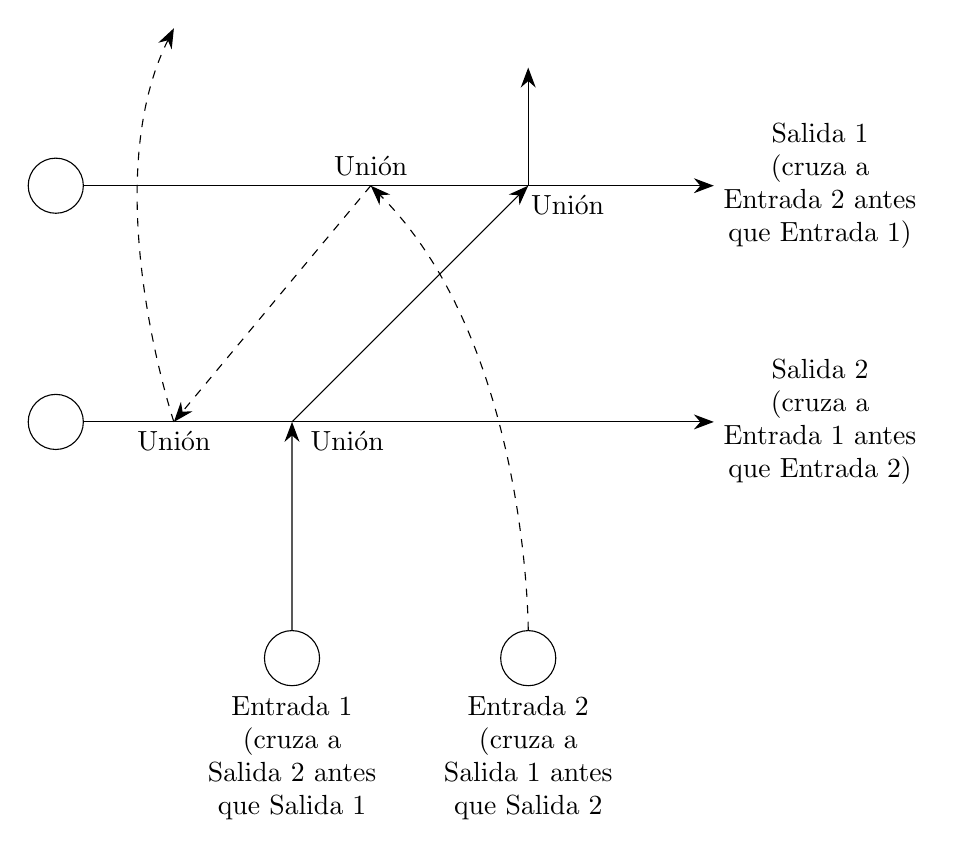
\begin{tikzpicture}
    \node[shape=circle, draw=black, minimum width=0.7cm, minimum height=0.7cm, inner sep=0pt] (A) at (0,0) {};
    \draw[-{Stealth[scale=1.5]}] (A.east) -- ++(8cm,0) node[right, align=center] {Salida 1\\ (cruza a \\ Entrada 2 antes \\ que Entrada 1)};

    \node[shape=circle, draw=black, minimum width=0.7cm, minimum height=0.7cm, inner sep=0pt] (B) at (0,-3) {};
    \draw[-{Stealth[scale=1.5]}] (B.east) -- ++(8cm,0) node[right, align=center] {Salida 2\\ (cruza a \\ Entrada 1 antes \\ que Entrada 2)};

    \node[shape=circle, draw=black, minimum width=0.7cm, minimum height=0.7cm, inner sep=0pt] (C) at (3,-6) {};
    \node[below, align=center] at (C.south) {Entrada 1\\(cruza a\\Salida 2 antes\\que Salida 1};
    \draw[-{Stealth[scale=1.5]}] (C.north) -- (3cm, -3cm);

    \node[shape=circle, draw=black, minimum width=0.7cm, minimum height=0.7cm, inner sep=0pt] (D) at (6,-6) {};
    \node[below, align=center] at (D.south) {Entrada 2\\(cruza a\\Salida 1 antes\\que Salida 2};
    \draw[dashed, -{Stealth[scale=1.5]}] (D.north) .. controls +(0,0) and +(2,-2) .. (4,0);

    \draw[dashed, -{Stealth[scale=1.5]}] (4, 0) -- (1.5, -3);

    \draw[dashed, -{Stealth[scale=1.5]}] (1.5, -3) .. controls +(0,0) and +(-1, -2) .. (1.5,2);

    \draw[-{Stealth[scale=1.5]}] (3, -3) -- (6, 0);

    \draw[-{Stealth[scale=1.5]}] (6, 0) -- (6, 1.5);

    \node[above] at (4, 0) {Unión};
    \node[below] at (1.5, -3) {Unión};
    \node[below] at (3.7, -3) {Unión};
    \node[below] at (6.5, 0) {Unión};
\end{tikzpicture}


\textbf{Figura 1.8} Un ejemplo con dos cables de entrada y dos cables de salida. La entrada 1 tiene su unión con la salida 2 aguas arriba de su unión con la salida 1; la entrada 2 tiene su unión con la salida 1 aguas arriba de su unión con la salida 2. Una solución válida es cambiar el flujo de datos de la entrada 1 a la salida 2, y el flujo de datos de la entrada 2 a la salida 1. Por otro lado, si el flujo de la entrada 1 se cambiara a la salida 1, y el flujo de la entrada 2 se cambiara a la salida 2, entonces ambos flujos pasarían a través de la caja de unión en el punto de encuentro de la entrada 1 y la salida 2 -- y esto no está permitido.\\

\textbf{Solución:} Un enrutamiento consiste precisamente en una correspondencia perfecta entre los cables de entrada y los cables de salida -- simplemente necesitamos elegir qué flujo de entrada será conmutado a qué cable de salida.\\

Desde el punto de vista de un cable de entrada, desea que su flujo de datos sea cambiado lo más temprano posible (cerca de la fuente): esto minimiza el riesgo de encontrarse con otro flujo de datos, que ya ha sido cambiado, en una caja de conexiones. Desde el punto de vista de un cable de salida, desea que un flujo de datos sea cambiado a él lo más tarde posible (lejos de la fuente): esto minimiza el riesgo de encontrarse con otro flujo de datos, que aún no ha sido cambiado, en una caja de conexiones.\\

Motivados por esta intuición, establecemos un problema de "matrimonio estable" que involucra a los cables de entrada y los cables de salida. Cada cable de entrada clasifica los cables de salida en el orden en que los encuentra desde la fuente hasta el terminal; cada cable de salida clasifica los cables de entrada en el orden inverso en que los encuentra desde la fuente hasta el terminal. Ahora mostramos:\\

\textit{Una emparejamiento estable entre los cables de entrada y los cables de salida define un cambio válido.} \\

Para demostrar esto, supongamos que este cambio hace que dos flujos de datos se crucen en una caja de conexiones. Supongamos que la caja de conexiones está en el punto de encuentro del cable de entrada $i$ y el cable de salida $j$. Entonces, uno de los flujos debe ser el que se origina en el cable de entrada $i$; el otro flujo debe haber cambiado desde un cable de entrada diferente, digamos el cable de entrada $k$, hacia el cable de salida $j$. Pero en este caso, el cable de salida $j$ prefiere el cable de entrada $i$ al cable de entrada $k$ (ya que $j$ se encuentra con $i$ más abajo que con $k$); y el cable de entrada $i$ prefiere el cable de salida $j$ al cable de salida, digamos el cable de salida $l$, al cual está realmente conectado -- ya que se encuentra con el cable de salida $j$ aguas arriba del Cable de salida . Esto contradice la suposición de que hemos elegido un emparejamiento estable entre los cables de entrada y los cables de salida.\\

Suponiendo que las intersecciones de los cables de entrada y los cables de salida están representadas por listas que contienen el orden en que cada cable se encuentra con los otros cables, podemos establecer las listas de preferencias para el problema del emparejamiento estable en tiempo $\mathcal{O}(n^2)$. Calcular el emparejamiento estable luego requiere tiempo adicional de $\mathcal{O}(n^2)$.
 

\newpage


\section{Notación Big O}
\section{Grafos}
\section{Greedy}
\section{Divide y venceras}
\section{Programación dinamica}
\section{Referencias}


\end{document}